% Bloque A: Pedro, 3:00. S1--S4. Problema y Design Thinking: perfil de
% usuaria, pregunta guía y lienzo de propuesta de valor.
\section{Problema y Design Thinking}
\begin{frame}
  \vspace{5mm}
  {\LARGE\color{colAcento}\bfseries ProductShot AI\par}
  \vspace{3mm}
  {\large\color{colAcento}Cinco ambientaciones para la foto de un producto,\\y una persona que decide cuáles usar\par}
  \vspace{8mm}
  Aaron Camacho, Nicolas Castañeda, Isaac Vera, Pedro Mori y Juan Diego Castro\par
  Planificación y Toma de Decisiones en IA (CS5363) --- UTEC 2026-2\par
  Docente: Robert Junior Buleje Del Carpio\par
  Noviembre de 2026
  \note{Pedro. 0:00--0:15 (15 s). Presentamos ProductShot AI: a partir de una
  foto casera de un producto, genera cinco ambientaciones para catálogo y
  redes, y una persona decide cuáles usaría. Primero el problema y la
  usuaria, luego la solución, los modelos, el agente y
  los resultados.}
\end{frame}

\begin{frame}{El problema: vender con fotos tomadas en casa}
  \begin{columns}[c]
    \begin{column}{0.30\textwidth}
      \centering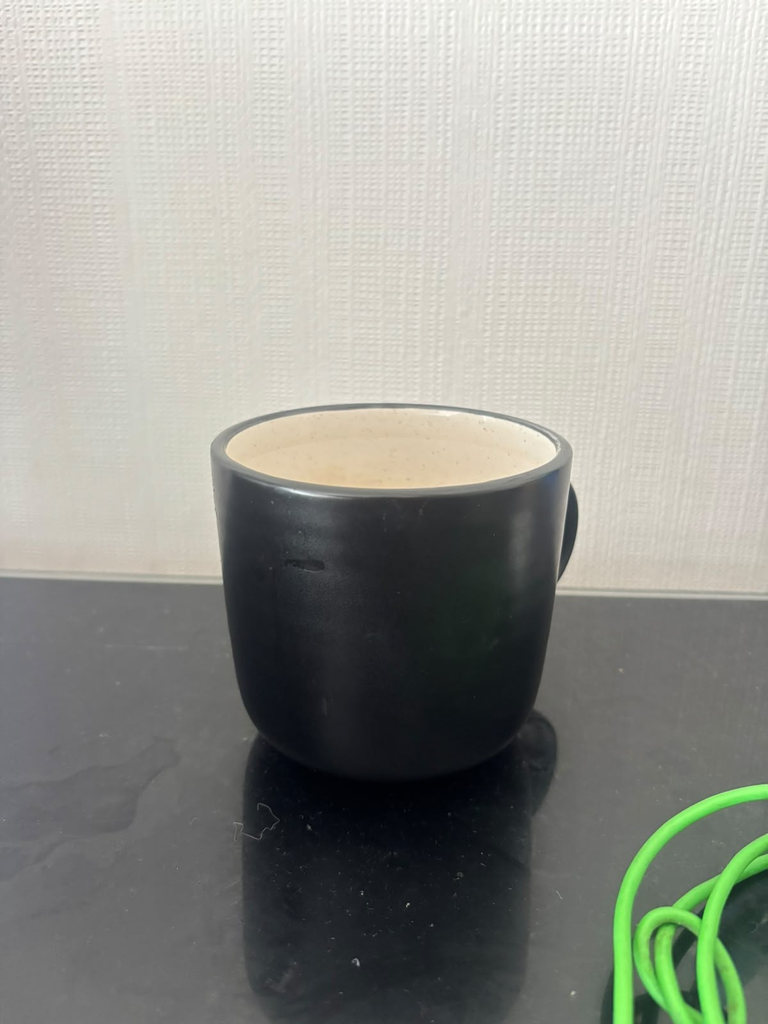
\includegraphics[height=5.2cm]{fig/input.png}\par
      {\scriptsize Foto casera de entrada}
    \end{column}
    \begin{column}{0.66\textwidth}\small
      \begin{itemize}\setlength{\itemsep}{6pt}
        \item Muchos emprendedores venden con fotos caseras, sin estudio ni experiencia en edición.
        \item Contratar un fotógrafo cada vez es caro y lento.
        \item Un fondo bonito no basta: la foto debe mostrar el producto
          \textbf{tal como es}, con su forma, su etiqueta y su logotipo.
      \end{itemize}
      \takeaway{El reto no es el fondo: es cambiar la escena sin cambiar el producto.}
    \end{column}
  \end{columns}
  \note{Pedro. 0:15--1:00 (45 s). Muchas personas venden por Instagram o
  Marketplace con fotos tomadas en casa, como esta taza. No tienen estudio
  ni saben editar, y un fotógrafo cada vez sale caro. Pero el reto no es
  solo poner un fondo bonito: una foto de venta tiene que mostrar el
  producto tal como es, con su forma, su etiqueta y su logo. Si la IA
  cambia el producto, la foto engaña al comprador. Esa tensión, cambiar la
  escena sin cambiar el producto, guía todo el diseño.}
\end{frame}

\begin{frame}{Design Thinking: ¿para quién lo hacemos?}
  \begin{columns}[T]
    \begin{column}{0.34\textwidth}\small
      \textbf{\color{colAcento}Perfil de usuaria}\par\smallskip
      \textbf{Vivian}, 32 años\\Emprendedora en Lima\par\medskip
      \textbf{Necesita} contenido que refleje la calidad real de sus
      productos y redes activas sin dedicarles mucho tiempo.\par\medskip
      \textbf{Quiere} hacer crecer su negocio y que su marca se vea como
      ella la imagina.
    \end{column}
    \begin{column}{0.30\textwidth}\small
      \textbf{\color{colWake}Frustraciones}
      \begin{itemize}\setlength{\itemsep}{4pt}
        \item No sabe de fotografía ni de edición.
        \item Un fotógrafo le resulta caro.
        \item Sus fotos no transmiten la calidad del producto.
      \end{itemize}
    \end{column}
    \begin{column}{0.30\textwidth}
      \begin{block}{Pregunta guía}
        \small ¿Cómo podríamos optimizar la generación de imágenes para un emprendedor?
      \end{block}
    \end{column}
  \end{columns}
  \source{Perfil construido por el equipo \textbf{sin usuarios reales}: lo contrastamos con una entrevista.}
  \note{Pedro. 1:00--2:00 (60 s). Representamos a la usuaria con un perfil:
  Vivian, 32 años, emprendedora en Lima. Necesita fotos que reflejen la calidad real de lo que vende y
  mantener sus redes activas sin perder horas. Sus frustraciones: no sabe
  de fotografía ni de edición, un fotógrafo le sale caro y sus fotos no
  transmiten la calidad del producto. La pregunta guía es: ¿cómo podríamos
  optimizar la generación de imágenes para un emprendedor? Un aviso
  honesto: el perfil lo construimos nosotros, sin usuarios reales. Por eso lo contrastamos con una entrevista, que
  Juan Diego presenta al final.}
\end{frame}

\begin{frame}{Lienzo de propuesta de valor: de frustración a decisión}
  \centering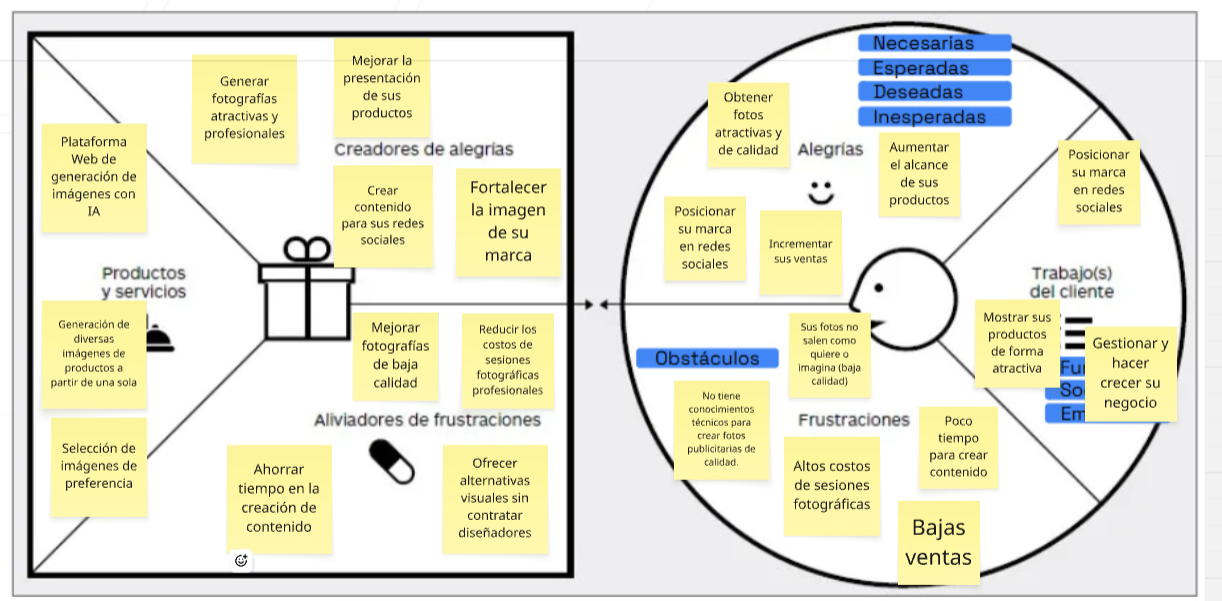
\includegraphics[width=0.58\textwidth]{fig/dt_lienzo.png}\par
  \smallskip\scriptsize
  \begin{tabular}{@{}ll@{}}
    \toprule
    Frustración o necesidad & Decisión de diseño \\
    \midrule
    Que la foto refleje la calidad real & Priorizar la fidelidad del producto (G8) \\
    Sin conocimientos técnicos & Solo subir una foto y aceptar o rechazar \\
    Costo y falta de tiempo & Una foto da cinco estilos por ronda \\
    \bottomrule
  \end{tabular}
  \note{Pedro. 2:00--3:00 (60 s). Este es el lienzo de propuesta de valor de
  ProductShot AI. A la derecha, el perfil: su trabajo es mostrar sus productos de
  forma atractiva y hacer crecer su negocio; sus frustraciones, costos
  altos, poco tiempo y fotos de baja calidad. A la izquierda, lo que
  ofrecemos: generar varias imágenes desde una sola foto y elegir las
  preferidas. Abajo, cómo se reflejan las frustraciones en el diseño. Que
  la foto muestre la calidad real lleva a priorizar la fidelidad. Sin
  conocimientos técnicos, la persona solo sube una foto y decide. Contra
  el costo y la falta de tiempo, una sola foto da cinco estilos. Lo que el
  lienzo promete sobre vender más o posicionar la marca queda fuera de lo
  que medimos. Aaron explica cómo funciona por dentro.}
\end{frame}
